\multiproblem{0}{{\it Basic work integrals} 
\newline
%For the following examples, calculate the work done on a particle of mass $m$ by each force.
\begin{enumerate}
\item A mass $m$ is released from a height $h$ above the ground. Calculate the work done by the gravitational force on the mass.
%
\item A mass $m$ is resting on a smooth surface and attached to a spring, the other end of which is attached to a wall. If the spring has natural length $L$ and spring constant $k$, calculate the work done on the mass when it is moved from position $P_1 = L$ to position $P_2 = 2L$.
%
\item A mass $m$ is constrained to move in an arc of radius $R$ on the surface of a table (ie. in a horizontal plane). Assume the table has a friction coefficient $\mu$. Calculate the work done by the friction force acting on the mass as it moves at constant velocity from $P_1 = (R,0)$ to $P_2 = (R,\pi)$, where positions are expressed in polar co-ordinates. 
{\it Hint: Friction always acts in the opposite direction to a particle's velocity}
\end{enumerate} 
}

\multiproblem{1}{{\it suvat equations and work}\newline
\begin{enumerate}
\item Considering the work-energy theorem and Newton's 2nd law, ${\bf F} = m{\bf a}$, derive the suvat equation for the final velocity $v$ of a mass $m$ moving in $1$ dimension given its initial velocity $u$, acceleration $a$ and displacement $s$: $$v^2 = u^2 + 2as.$$
%
\A{$\Delta T = \frac{1}{2}mv^2 - \frac{1}{2}mu^2 = W = F\Delta r = mas \to  \frac{1}{2}mv^2 - \frac{1}{2}mu^2 = mas$}
%
\A{Re-arranging and dividing through by $m$: $v^2 = u^2 + 2as$}
%
\item Repeat the above for a particle moving in $2$ or $3$ dimensions.
%
\A{$\Delta T = \frac{1}{2}m|{\bf v}|^2 - \frac{1}{2}m|{\bf u}|^2 = 2{\bf a}\cdot{\bf s}$}
\end{enumerate}
}


\multiproblem{2}{{\it Work and a parabolic trajectory}\newline
Consider a mass $m$ projected with velocity $v_0$ at an angle $\alpha$ from the origin in the $x-z$ plane.

	\begin{center}
                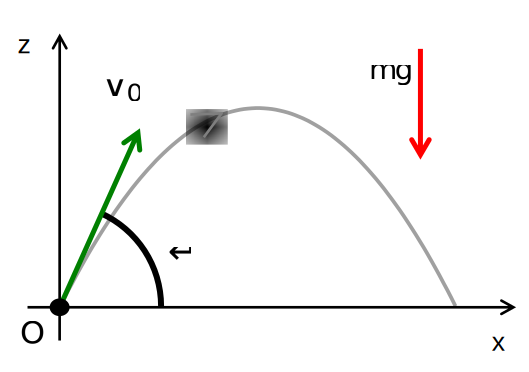
\includegraphics[scale=0.4]{parabola.pdf}
         \end{center}

\begin{enumerate}
\item Using N2L, write down force vector ${\bf F}(t)$.
%
\A{${\bf F}(t) = (0,0,-mg)$}
%
\item Using your expression for ${\bf F}(t)$, find expressions for ${\bf v}(t)$ and ${\bf r}(t)$, the velocity and position vectors of the particle.
%
\A{${\bf v}(t) = (v_0\cos\alpha,0,v_0\sin\alpha - gt)$}
\A{${\bf r}(t) = (tv_0\cos\alpha,0,tv_0\sin\alpha - \frac{1}{2}gt^2)$}
%
\item Calculate the work done by ${\bf F}(t)$ as a function of time, $W(t)$. What do you notice about the terms in your final expression?
\A{$F(t)\cdot dr = {\bf F}(t)\cdot {\bf v}(t)dt = -mgv_0\sin\alpha + mg^2t$}
\A{$W = \int {\bf F}(t)\cdot {\bf v}(t)dt = -mgtv_0\sin\alpha + \frac{1}{2}m(gt)^2$}
%
\item Using your knowledge about the conservation of energy, determine an expression for $z_{max}$, the maximum height the mass would reach during its trajectory.
\A{$\frac{1}{2}mv_0^2 = mgz_{max} \to z_{max} = \frac{1}{2g}v_0^2$}
%
\item Using your knowledge about different types of forces, determine the time it would take for the mass to complete its trajectory (ie. ${\bf r}(t) = (x,0,0)$, $x > 0$)
\A{$t = \frac{2}{mg}v_0\sin\alpha$}
%
\end{enumerate}
}

\multiproblem{3}{{\it Mass on a smooth slope}\newline
Consider mass $m$ on a smooth slope at an angle $\alpha$ to the horizontal.
\bigskip
	\begin{center}
                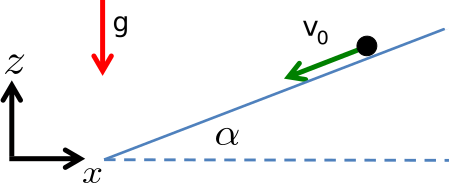
\includegraphics[scale=0.4]{slope.pdf}
         \end{center}
\bigskip
\begin{enumerate}
\item Draw a free body diagram for the mass. Which, if any, are forces of constraint?
%
%\item If the mass is stationary, which forces acting on the mass are forces of constraint?
% 
\item If the mass moves from position ${\bf r}_0$ to ${\bf r}_1$, how much work is done on the mass? If it then moves back to ${\bf r}_0$, what is the total amount of work that has been done?
%
\A{From ${\bf r}_0$ to ${\bf r}_1$, $W_{01} = V({\bf r}_1) - V({\bf r}_0 = -mg(z_1 - z_0))$}
\A{From ${\bf r}_1$ to ${\bf r}_0$, $W =_{10} V({\bf r}_0) - V({\bf r}_1 = -mg(z_0 - z_1))$}
\A{$W_{01}+W_{10} = 0.$ The only force acting is the gravitational force which is conservative.}
%
\item If the mass is released from position ${\bf r}(0) = (x_0,0,z_0)$ with initial velocity $v_0$, calculate its later position as a function of time, ${\bf r}(t)$.
%
%ANSWER
\A{${\bf F}(t) = (0,0, -mg)$}
\A{${\bf v}(t) = \int{\bf a}(t)dt + {\bf v}_0 = (0,0,-gt) + (v_0\cos\alpha, 0, -v_0\sin\alpha)$ }
\A{${\bf r}(t) = \int{\bf v}(t)dt + {\bf r}(0) = (v_0t\cos\alpha, 0, -v_0t\sin\alpha - \frac{1}{2}gt^2) + (x_0,0,z_0)$}
%
\item Using the work-energy theorem, calculate the work done on the mass as it moves from ${\bf r}(0)$ to ${\bf r}(t)$.
%
%ANSWER
\A{Using work-energy theorem, $W = \Delta T$}
\A{$\Delta T = \frac{1}{2}m(|{\bf v}(t)|^2 - |{\bf v}(0)|^2)$}
\A{$\Delta T = \frac{1}{2}m (v_0^2 + 2v_0gt \sin\alpha + (gt)^2 - v_0^2) =  \frac{1}{2}m (2v_0gt \sin\alpha + (gt)^2)$} 
%
\item In order to verify the work-energy theorem, calculate the work done on the mass as it moves from  ${\bf r}(0)$ to ${\bf r}(t)$ by explicit calculation (ie. $W = \int {\bf F}\cdot d{\bf r} \equiv \int {\bf F}\cdot {\bf v} dt$). 
%
%ANSWER
\A{Can use either ${\bf v}(t)$ or ${\bf r}(t)$. If ${\bf v}(t)$ is used:}
\A{$W = \int {\bf F}\cdot {\bf v} dt = m \int {\bf a}\cdot{\bf v} dt = m \int g v_0\sin\alpha + g^2t = m (gtv_0\sin\alpha + \frac{1}{2}(gt)^2$.
}
\end{enumerate}
}

\multiproblem{4}{{\it Mass on a rough slope}\newline

Now assume that mass $m$ is on a rough slope, with coefficient of friction $\mu$.
\begin{enumerate}
\item If the mass is stationary (not slipping), which forces acting on the mass are forces of constraint?
%
\item Using force balance, write an equation for the net force parallel to the slope acting on the mass when it is stationary.
%
\item Now assume the mass is slipping. How much work is done on the mass moving it from ${\bf r}_0$ to ${\bf r}_1$? If it then moves back to ${\bf r}_0$, what is the total amount of work that has been done?
%
\item Using your expression for the net force, determine expressions for the velocity and position of the mass as functions of time, $v(t)$ and $r(t)$.
\item If the mass is given an initial velocity $v_0$ acting down the slope, calculate the work done on the mass by the friction force to bring it to rest.
\item Calculate the total work done on the mass by all forces to bring it to rest.
\item Repeat the above two questions with the initial velocity $v_0$ acting up the slope. How does your answer differ and why?
\end{enumerate}
}

\multiproblem{5}{{\it Mass on a (hypothetical) rollercoaster}\newline
Consider a mass $m$ moving at velocity $v_0$ towards a rollercoaster loop of radius $R$. When it is at the top of the loop, its velocity will be $v_1$. Assume the rollercoaster track has no friction.

	\begin{center}
                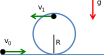
\includegraphics[scale=0.4]{coaster.pdf}
         \end{center}
         
\begin{enumerate}
\item Draw a free body diagram of the mass when it is at the top of the loop. 
\item From your free body diagram, write down an inequality for the normal reaction, $N$, being exerted on the mass by the rollercoaster track.
%
\A{At the top of the loop, $N \geq 0$. From force balance we have $N + mg = \frac{mv_1^2}{R}.$}
\A{Hence, $\frac{mv_1^2}{R} - mg \geq 0$. Rearranging gives $v_1^2 \geq gR$.
}
%
\item Using this inequality along with what you know about conservative forces, determine the minimum value of $v_0$, as a function of $g$ and $R$, which ensures the mass will not leave the track as it passes through the loop. 
%
\A{Only conservative forces acting so energy is conserved.}
\A{$E = \frac{1}{2}mv_0^2 = \frac{1}{2}mv_1^2 + 2mgR$}
\A{Rearrange for $v_1^2$ and substitute into the inequality from the previous part: $v_0^2 - 4gR \geq gR$.}
\A{Minimum value of $v_0$ is thus $v_0 = \sqrt{5gR}$.}
\end{enumerate}
}